\documentclass[conference]{IEEEtran}
\IEEEoverridecommandlockouts

\usepackage{cite}
\usepackage{amsmath,amssymb,amsfonts}
\usepackage{graphicx}
\usepackage{textcomp}
\usepackage{xcolor}
\usepackage{booktabs}
\usepackage{url}
\usepackage{tikz}
\usetikzlibrary{shapes.geometric, arrows.meta, positioning, fit, backgrounds}

\definecolor{boxblue}{RGB}{235, 243, 250}
\definecolor{borderblue}{RGB}{31, 110, 180}
\definecolor{boxgreen}{RGB}{235, 247, 238}
\definecolor{bordergreen}{RGB}{46, 139, 87}
\definecolor{boxorange}{RGB}{254, 243, 235}
\definecolor{borderorange}{RGB}{210, 105, 30}
\definecolor{boxpurple}{RGB}{245, 238, 252}
\definecolor{borderpurple}{RGB}{128, 0, 128}
\definecolor{boxgray}{RGB}{245, 245, 245}
\definecolor{bordergray}{RGB}{120, 120, 120}

\begin{document}

\title{Open Source Companion: An Intelligent Platform for Personalized Open-Source Contribution Onboarding and Issue Recommendation}

\author{
\IEEEauthorblockN{Rahul S\IEEEauthorrefmark{1}, Contributor Two\IEEEauthorrefmark{2}, and Contributor Three\IEEEauthorrefmark{3}}
\IEEEauthorblockA{Department of Computer Science and Engineering\\
MVJ College of Engineering, Bengaluru, India\\
Email: \{rahul.s, contributor2, contributor3\}@mvjce.edu.in}
}

\maketitle

\begin{abstract}
Open-source software (OSS) ecosystems depend fundamentally on sustainable newcomer onboarding, yet aspiring contributors face steep barriers, including difficulty locating beginner-appropriate tasks, navigating unfamiliar project landscapes, and managing contribution lifecycles. Existing repository hosting interfaces offer coarse issue labeling that lacks personal skill alignment and structured workflow guidance. This paper presents \textit{Open Source Companion}, an integrated, full-stack platform designed to facilitate newcomer onboarding through automated issue acquisition, interpretable heuristic difficulty categorization, contributor skill profiling, and a guided six-stage contribution workflow. The implemented system incorporates real-time GitHub Search API ingestion, OAuth-based profile extraction from contributor repositories, transparent multi-factor matching, pull-request readiness analysis, and milestone-based gamification backed by a PostgreSQL database and Prisma ORM. We formalize the issue characterization and matching methodology, report system validation demonstrating end-to-end architectural feasibility, and formulate an extensible machine-learning research framework together with a reproducible empirical benchmark protocol for future learned classification and dense semantic retrieval.
\end{abstract}

\begin{IEEEkeywords}
Open-source software, GitHub, issue recommendation, contributor onboarding, software engineering, machine learning, gamification, contribution tracking.
\end{IEEEkeywords}

\section{Introduction}
Open-source software (OSS) has evolved into the bedrock of modern computing infrastructure, underpinning operating systems, cloud frameworks, and machine-learning platforms~\cite{mockus2002two}. The long-term vitality of these projects relies on continuously attracting, onboarding, and retaining new contributors~\cite{steinmacher2015systematic}. However, the transition from an interested developer to an active open-source contributor involves substantial friction. Empirical studies demonstrate that newcomers frequently abandon their contribution attempts due to complex technical environments, information overload, and difficulty identifying appropriately scoped tasks~\cite{steinmacher2015systematic, dagenais2010moving}.

While repository platforms such as GitHub provide task tags (e.g., \texttt{good first issue}, \texttt{help wanted}), these labels suffer from well-documented limitations: they are assigned manually, vary widely in quality across repositories, become stale rapidly, and fail to account for a newcomer's individual background and technical skill set~\cite{tan2020first, xiao2022recommending}. Furthermore, once a potential task is identified, newcomers face secondary barriers: configuring local development environments, adhering to project-specific coding conventions, crafting acceptable pull requests (PRs), and tracking contribution reviews~\cite{storey2017social}. Conventional tools address these stages in isolation, leaving contributors to navigate fragmented resources across issue trackers, documentation wikis, and git command-line interfaces~\cite{steinmacher2016overcoming}.

This paper presents \textit{Open Source Companion}, an end-to-end intelligent platform engineered to unify issue discovery, transparent difficulty characterization, contributor modeling, guided task execution, and progress tracking. The platform operates on a production-grade full-stack architecture built with Next.js~16, React~19, TypeScript, PostgreSQL~15, Prisma~ORM, and Auth.js~v5. The system ingests live GitHub issues, categorizes difficulty via transparent metadata heuristics, derives contributor skill profiles during OAuth authentication, provides a multi-stage contribution workspace, and maintains long-term engagement via gamified milestones.

To ensure research integrity, this work explicitly distinguishes between the \textit{implemented system} and \textit{proposed research extensions}. The implemented system delivers deterministic, rule-based categorization, multi-factor recommendation drawers, and a six-stage contribution workflow. We complement this operational platform by designing an extensible machine-learning framework that defines how supervised classifiers (e.g., XGBoost, Random Forest) and dense semantic vector retrieval (Sentence-BERT, FAISS) can be integrated, accompanied by a reproducible evaluation protocol.

The main contributions of this work are:
\begin{enumerate}
    \item \textbf{Integrated Platform Architecture:} An end-to-end system architecture integrating GitHub issue discovery, contributor profiling, structured contribution guidance, contribution tracking, and gamification within a unified platform.
    \item \textbf{Interpretable Issue Characterization:} A transparent rule-based issue difficulty categorization mechanism based on available GitHub metadata and labels, providing understandable difficulty tiers for newcomers.
    \item \textbf{Contributor-Aware Issue Matching:} A contributor-aware recommendation workflow that combines contributor skill profiles with issue characteristics to identify potentially suitable contribution opportunities.
    \item \textbf{Structured Contribution Lifecycle:} A six-stage contribution workflow that guides a contributor from issue understanding through repository setup, implementation, commit preparation, pull-request preparation, and merge verification.
    \item \textbf{Extensible ML Research Framework:} A proposed extension path for replacing heuristic categorization and matching with learned models and dense semantic retrieval, together with a reproducible evaluation protocol.
\end{enumerate}

The remainder of this paper is organized as follows: Section~II reviews related work and presents a comparative taxonomy. Section~III formulates the research problem and states the research questions. Section~IV details the system methodology. Section~V outlines the software architecture. Section~VI provides system validation and the proposed ML evaluation protocol. Section~VII discusses trade-offs. Section~VIII examines threats to validity, Section~IX addresses ethical aspects, and Section~X concludes the paper.

\section{Related Work}

\subsection{Open-Source Newcomer Onboarding}
Newcomer onboarding in OSS has received substantial attention in software engineering literature. In a foundational systematic literature review, Steinmacher et al.~\cite{steinmacher2015systematic} identified 15 distinct barriers grouped into technical hurdles, documentation shortcomings, social interaction friction, previous knowledge gaps, and orientation difficulties. Dagenais et al.~\cite{dagenais2010moving} studied the project landscape newcomers navigate, noting that early validation of progress is vital for sustained participation. To mitigate onboarding barriers, Steinmacher et al.~\cite{steinmacher2016overcoming} developed FLOSScoach, a portal organizing contribution activities. While FLOSScoach established the value of structured orientation, it operated largely as a static informational portal without direct integration into repository issue tracking or automated personal profile matching.

\subsection{Issue and Task Recommendation}
Automated task recommendation has been explored through various lenses. Early work by Anvik et al.~\cite{anvik2006who} applied supervised classifiers to triage incoming bug reports to experienced developers. Cubranic et al.~\cite{cubranic2005hipikat} created Hipikat, which recommended artifacts based on historical project memory. More recently, Xiao et al.~\cite{xiao2022recommending} developed RecGFI to recommend ``good first issues'' using XGBoost on issue textual features and historical dynamics, while Tan et al.~\cite{tan2020first} empirically analyzed how GFI labels are utilized on GitHub. He et al.~\cite{he2023personalized} proposed PFIRec, demonstrating that generic beginner labels often mismatch newcomer backgrounds and that personalized recommendation is necessary. While these studies advanced predictive modeling, they focused on the recommendation step in isolation without providing an operational execution environment.

\subsection{Issue Difficulty and Effort Estimation}
Predicting issue resolution complexity and effort is critical for realistic task assignment. Kikas et al.~\cite{kikas2016using} leveraged dynamic and contextual features to predict issue lifetime across over 4,000 GitHub projects using tree-based ensembles. Zhou et al.~\cite{zhou2012where} utilized information retrieval techniques for bug localization, demonstrating the predictive power of issue textual tokens. Existing difficulty estimators, however, often produce black-box numerical outputs that lack actionable, transparent explanations for newcomers.

\subsection{Gamification and Developer Engagement}
Gamification has been studied as a mechanism to sustain contributor motivation. Pedreira et al.~\cite{pedreira2015gamification} mapped gamification techniques in software engineering, identifying points, badges, and leaderboards as predominant engagement tools. Vasilescu et al.~\cite{vasilescu2014social} examined how badge-based reputation systems influence knowledge exchange on Stack Overflow and GitHub, while Singer and Schneider~\cite{singer2012race} observed that lightweight gamification can stimulate active version control usage.

\subsection{Research Gap}
Existing studies have addressed individual aspects of newcomer onboarding, task recommendation, issue characterization, and contributor engagement. The present work explores their integration into a unified contribution workflow, bridging the transition from initial task discovery to step-by-step local implementation, PR submission, and verified milestone progression, as summarized in Table~\ref{tab:comparison}.

\begin{table*}[t]
\caption{Comparison with Existing Approaches}
\label{tab:comparison}
\centering
\scriptsize
\setlength{\tabcolsep}{3pt}
\begin{tabular}{@{}lp{2.3cm}p{2.5cm}p{2.3cm}p{2.4cm}p{2.3cm}p{1.9cm}@{}}
\toprule
\textbf{Approach} & \textbf{Newcomer Support} & \textbf{Issue Recommendation} & \textbf{Difficulty Estimation} & \textbf{Contributor Modeling} & \textbf{Contribution Workflow} & \textbf{Gamification} \\
\midrule
FLOSScoach~\cite{steinmacher2016overcoming} & Comprehensive & None & None & None & Informational portal & None \\
Hipikat~\cite{cubranic2005hipikat} & Incidental & Artifact recommendation & None & Historical artifact links & None & None \\
RecGFI~\cite{xiao2022recommending} & Targeted to GFIs & Binary classification & Binary (GFI vs. non-GFI) & None & None & None \\
PFIRec~\cite{he2023personalized} & Personalized & Content-based ranking & Relative ranking & Activity history & None & None \\
Issue Lifetime~\cite{kikas2016using} & None & None & Continuous duration & None & None & None \\
\textbf{Open Source Companion} & \textbf{End-to-end} & \textbf{Rule-based multi-factor} & \textbf{Interpretable 3-tier} & \textbf{GitHub language profile} & \textbf{6-stage guided path} & \textbf{Points, badges, streaks} \\
\bottomrule
\end{tabular}
\end{table*}

\section{Problem Formulation and Objectives}

\subsection{Mathematical Formulation}
Let $\mathcal{I} = \{i_1, i_2, \dots, i_N\}$ denote the set of open GitHub issues ingested from public repositories. Each issue $i \in \mathcal{I}$ is represented by an attribute tuple:
\begin{equation}
\mathbf{x}_i = \langle \tau_i, \beta_i, \mathcal{L}_i, \rho_i, c_i \rangle
\end{equation}
where $\tau_i$ represents the issue title, $\beta_i$ denotes the issue body text, $\mathcal{L}_i = \{l_{i,1}, \dots, l_{i,m}\}$ is the set of assigned label strings, $\rho_i$ denotes the parent repository identifier, and $c_i \in \mathbb{N}$ denotes the comment count.

Let $\mathcal{U}$ denote the set of registered contributors. A contributor $u \in \mathcal{U}$ is modeled as:
\begin{equation}
\mathbf{p}_u = \langle \mathbf{s}_u, e_u, \mathcal{H}_u, \kappa_u \rangle
\end{equation}
where $\mathbf{s}_u = \{(g, w_{u,g}) \mid g \in \mathcal{G}\}$ represents a normalized programming language profile derived from public repositories, $e_u \in \{\text{Beginner}, \text{Intermediate}, \text{Advanced}\}$ represents self-declared experience, $\mathcal{H}_u$ represents active contribution records, and $\kappa_u \in \mathbb{N}$ represents accumulated points.

The system addresses two sequential mappings:
\begin{enumerate}
    \item \textbf{Difficulty Categorization:} A function $\Phi: \mathbf{x}_i \to d_i$, where $d_i \in \{\text{Beginner}, \text{Intermediate}, \text{Advanced}\}$.
    \item \textbf{Personalized Matching:} A scoring function $S(u, i) \in [0, 100]$ ranking candidates for contributor $u$.
\end{enumerate}

In the implemented prototype, the composite recommendation score $S(u,i)$ in the interactive drawer is computed as:
\begin{equation}
\begin{split}
S(u, i) = \;& \lambda_1 M_{\text{skill}}(u, i) + \lambda_2 M_{\text{diff}}(u, i) \\
& + \lambda_3 M_{\text{repo}}(i) + \lambda_4 M_{\text{sem}}(u, i)
\end{split}
\label{eq:scoring}
\end{equation}
where $M_{\text{skill}}$ measures language alignment, $M_{\text{diff}}$ assesses tier compatibility, $M_{\text{repo}}$ reflects repository activity, and $M_{\text{sem}}$ denotes heuristic semantic overlap, with equal default weight distribution $\sum_{k=1}^4 \lambda_k = 1.0$.

\subsection{Research Questions}
To investigate this integrated platform, we state three core research questions:
\begin{itemize}
    \item \textbf{RQ1:} How can publicly available GitHub issue metadata and labeling information be used to provide interpretable difficulty categorization for open-source newcomers?
    \item \textbf{RQ2:} How can contributor profiles derived from public repository activity be combined with issue characteristics to generate interpretable issue recommendations?
    \item \textbf{RQ3:} How can a structured, phased contribution workflow integrate issue discovery, repository setup, implementation guidance, pull-request preparation, and contribution verification into a unified onboarding process?
\end{itemize}

\section{Proposed System Methodology}

\begin{figure}[t]
\centering
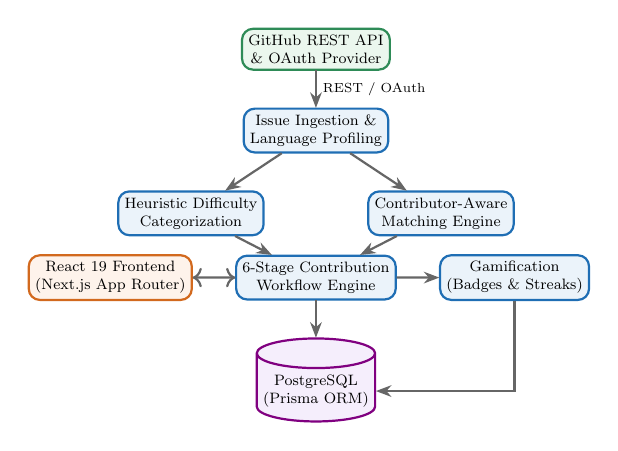
\begin{tikzpicture}[
    scale=0.68, every node/.style={transform shape},
    node distance=0.7cm and 0.7cm,
    block/.style={rectangle, draw=borderblue, fill=boxblue, thick, rounded corners, align=center, minimum height=0.7cm, minimum width=2.1cm, font=\footnotesize},
    extblock/.style={rectangle, draw=bordergreen, fill=boxgreen, thick, rounded corners, align=center, minimum height=0.7cm, minimum width=2.1cm, font=\footnotesize},
    dbblock/.style={cylinder, shape border rotate=90, draw=borderpurple, fill=boxpurple, thick, aspect=0.25, align=center, minimum height=0.85cm, minimum width=2.0cm, font=\footnotesize},
    ui/.style={rectangle, draw=borderorange, fill=boxorange, thick, rounded corners, align=center, minimum height=0.7cm, minimum width=2.1cm, font=\footnotesize},
    arrow/.style={-{Stealth[scale=0.85]}, thick, draw=gray!80!black}
]
    \node[extblock] (gh) {GitHub REST API\\\& OAuth Provider};
    
    \node[block, below=0.7cm of gh] (ingest) {Issue Ingestion \&\\Language Profiling};
    
    \node[block, below left=0.7cm and -0.4cm of ingest] (diff) {Heuristic Difficulty\\Categorization};
    \node[block, below right=0.7cm and -0.4cm of ingest] (rec) {Contributor-Aware\\Matching Engine};
    
    \node[block, below=1.9cm of ingest] (flow) {6-Stage Contribution\\Workflow Engine};
    
    \node[dbblock, below=0.7cm of flow] (db) {PostgreSQL\\(Prisma ORM)};
    
    \node[ui, left=0.8cm of flow] (ui_view) {React 19 Frontend\\(Next.js App Router)};
    \node[block, right=0.8cm of flow] (game) {Gamification\\(Badges \& Streaks)};

    \draw[arrow] (gh) -- node[right, font=\scriptsize] {REST / OAuth} (ingest);
    \draw[arrow] (ingest) -- (diff);
    \draw[arrow] (ingest) -- (rec);
    \draw[arrow] (diff) -- (flow);
    \draw[arrow] (rec) -- (flow);
    \draw[arrow] (flow) -- (db);
    \draw[arrow] (flow) -- (game);
    \draw[arrow] (game) |- (db);
    \draw[arrow, <->] (ui_view) -- (flow);
\end{tikzpicture}
\caption{System Architecture of Open Source Companion, showing data acquisition from GitHub, application logic layers, persistence, and user interfaces.}
\label{fig:arch}
\end{figure}

\subsection{System Overview}
The overall architecture of Open Source Companion is depicted in Fig.~\ref{fig:arch}. External communication with GitHub is mediated via HTTPS using the GitHub REST API v3 and OAuth~2.0. Ingested data feeds into internal processing services that execute issue difficulty categorization, contributor profile synthesis, recommendation scoring, and state-machine transitions across the contribution lifecycle.

\subsection{Issue Data Collection and Ingestion}
Issue data is collected through the GitHub Search API using the query:
\begin{equation*}
\textstyle \mathtt{q = is:issue + is:open + label:"help~wanted"}
\end{equation*}
sorted by most recent updates. When a valid \texttt{GITHUB\_TOKEN} is configured, requests execute under authenticated rate limits (5,000 requests/hour), while unauthenticated fallbacks operate under standard limits (60 requests/hour).

Ingested JSON payloads are normalized into the application domain model. Repository identifiers are extracted from the API URI ($\rho_i = \text{owner}/\text{repo}$), titles and bodies are sanitized, and issue labels are parsed into lowercase sets for downstream categorization.

\subsection{Interpretable Issue Difficulty Categorization}
Rather than deploying an unverified black-box model, the operational platform implements an interpretable rule-based categorization heuristic $\Phi(\mathbf{x}_i)$. Let $\mathcal{L}_i^{\text{low}}$ denote the normalized set of lowercase labels for issue $i$:
\begin{equation}
\Phi(\mathbf{x}_i) = 
\begin{cases}
\text{Beginner}, & \text{if } \mathcal{L}_i^{\text{low}} \cap \mathcal{K}_{\text{beg}} \neq \emptyset \\
\text{Advanced}, & \text{if } \mathcal{L}_i^{\text{low}} \cap \mathcal{K}_{\text{adv}} \neq \emptyset \\
\text{Intermed.}, & \text{otherwise (modulo distribution)}
\end{cases}
\end{equation}
where $\mathcal{K}_{\text{beg}} = \{\text{``good first issue''}, \text{``first-timers-only''}\}$ and $\mathcal{K}_{\text{adv}} = \{\text{``enhancement''}, \text{``feature''}\}$. Unlabeled or ambiguous issues default to an intermediate baseline with cyclic round-robin distribution to maintain diverse exploratory options.

Each categorized tier maps deterministically to an estimated completion effort and gamified point value:
\begin{itemize}
    \item \textbf{Beginner:} Effort: 1--3 hours; Reward: 50 points.
    \item \textbf{Intermediate:} Effort: 3--8 hours; Reward: 150 points.
    \item \textbf{Advanced:} Effort: 1--3 days; Reward: 300 points.
\end{itemize}

\subsection{Contributor Modeling}
Contributor profiling occurs seamlessly during OAuth authentication. During the \texttt{jwt} callback in Auth.js, the system queries the authenticated contributor's repository endpoint:
\begin{equation*}
\texttt{GET /user/repos?sort=updated\&per\_page=10}
\end{equation*}
The platform aggregates the primary language tags across these repositories, computes frequency distributions, and extracts the top five languages to populate $\mathbf{s}_u$. Contributors can also refine their technical interests, bio, and declared experience tier ($e_u$) via their profile settings.

\subsection{Six-Stage Contribution Lifecycle}
The core onboarding mechanism is a structured six-stage contribution workflow designed to decompose complex software tasks into explicit, manageable steps:
\begin{enumerate}
    \item \textbf{Stage 1: Understand.} The contributor inspects the issue description, maintainer commentary, and a pre-flight checklist verifying affected components and test requirements.
    \item \textbf{Stage 2: Setup.} The platform generates repository-specific git commands for cloning the remote repository, navigating into the workspace, and creating an isolated feature branch.
    \item \textbf{Stage 3: Implement.} The contributor performs code modifications guided by contextual code snippets and an implementation checklist.
    \item \textbf{Stage 4: Commit.} The platform generates conventional commit message templates referencing the originating issue number (e.g., \texttt{fix: improve validation; Closes \#421}).
    \item \textbf{Stage 5: Pull Request Preparation.} The contributor prepares PR metadata and reviews readiness signals (scope alignment, test coverage, repository fit).
    \item \textbf{Stage 6: Merge \& Verification.} The platform validates that the contributor has forked the repository, records PR submission state, updates contribution status, and triggers point allocation upon merge verification.
\end{enumerate}

\begin{figure}[t]
\centering
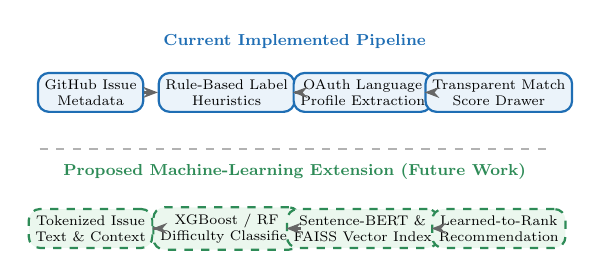
\begin{tikzpicture}[
    scale=0.72, every node/.style={transform shape},
    node distance=0.55cm and 0.5cm,
    impproc/.style={rectangle, draw=borderblue, fill=boxblue, thick, rounded corners, align=center, font=\scriptsize, minimum height=0.65cm},
    propproc/.style={rectangle, draw=bordergreen, fill=boxgreen, thick, dashed, rounded corners, align=center, font=\scriptsize, minimum height=0.65cm},
    arrow/.style={-{Stealth[scale=0.8]}, thick, draw=gray!80!black}
]
    % Implemented Pipeline
    \node[font=\footnotesize\bfseries, text=borderblue] (imp_label) at (0, 3.7) {Current Implemented Pipeline};
    \node[impproc] (raw1) at (-3.6, 2.8) {GitHub Issue\\Metadata};
    \node[impproc] (heur) at (-1.2, 2.8) {Rule-Based Label\\Heuristics};
    \node[impproc] (prof1) at (1.2, 2.8) {OAuth Language\\Profile Extraction};
    \node[impproc] (out1) at (3.6, 2.8) {Transparent Match\\Score Drawer};
    
    \draw[arrow] (raw1) -- (heur);
    \draw[arrow] (heur) -- (prof1);
    \draw[arrow] (prof1) -- (out1);

    % Divider
    \draw[dashed, gray!60, thick] (-4.5, 1.8) -- (4.5, 1.8);

    % Proposed ML Pipeline
    \node[font=\footnotesize\bfseries, text=bordergreen] (prop_label) at (0, 1.4) {Proposed Machine-Learning Extension (Future Work)};
    \node[propproc] (raw2) at (-3.6, 0.4) {Tokenized Issue\\Text \& Context};
    \node[propproc] (ml) at (-1.2, 0.4) {XGBoost / RF\\Difficulty Classifier};
    \node[propproc] (sbert) at (1.2, 0.4) {Sentence-BERT \&\\FAISS Vector Index};
    \node[propproc] (rank) at (3.6, 0.4) {Learned-to-Rank\\Recommendation};

    \draw[arrow] (raw2) -- (ml);
    \draw[arrow] (ml) -- (sbert);
    \draw[arrow] (sbert) -- (rank);
\end{tikzpicture}
\caption{Comparison between the currently implemented heuristic pipeline and the proposed machine-learning research extension.}
\label{fig:pipeline_comp}
\end{figure}

\subsection{Gamification and Progress Tracking}
To sustain newcomer motivation without creating perverse incentives, gamification elements are directly coupled to verified milestone transitions. The system manages:
\begin{itemize}
    \item \textbf{Accumulated Points:} Awarded upon issue enrollment (25 points) and successful PR merge (50--300 points based on difficulty).
    \item \textbf{Milestone Badges:} Automated evaluation unlocks badges including \texttt{first\_issue}, \texttt{first\_pr}, \texttt{three\_prs}, \texttt{contributions\_10}, \texttt{week\_warrior}, and streak milestones.
    \item \textbf{Global Leaderboard:} Contributor rankings computed dynamically via PostgreSQL queries ordered by points descending and streak days descending.
\end{itemize}

\subsection{Proposed Machine-Learning Extension}
While the operational platform relies on deterministic rules, its modular architecture permits drop-in replacement with learned components, as illustrated in Fig.~\ref{fig:pipeline_comp}:
\begin{itemize}
    \item \textbf{Difficulty Classification:} Replacing rule heuristics with an XGBoost~\cite{chen2016xgboost} or Random Forest~\cite{breiman2001random} model trained on textual TF-IDF features, issue age, comment volume, and code-block ratios.
    \item \textbf{Semantic Embedding \& Retrieval:} Encoding issue descriptions and developer interest vectors using Sentence-BERT~\cite{reimers2019sentence}, indexed via FAISS~\cite{johnson2021billion} for sub-second approximate nearest neighbor retrieval over large issue corpora.
    \item \textbf{Learning-to-Rank:} Formulating candidate ranking via LambdaMART or coordinate ascent incorporating implicit historical interaction signals.
\end{itemize}

\section{Software Architecture and Data Tier}
The platform is implemented using modern web and systems technologies. Next.js~16 utilizes React~19 Server Components and asynchronous Server Actions to eliminate redundant REST boilerplate while preserving type safety between client interfaces and persistence tiers.

\begin{table}[t]
\caption{Database Schema Entities in PostgreSQL via Prisma ORM}
\label{tab:schema}
\centering
\scriptsize
\setlength{\tabcolsep}{2.5pt}
\begin{tabular}{@{}lp{1.8cm}p{4.2cm}@{}}
\toprule
\textbf{Entity} & \textbf{Key Fields} & \textbf{Description and Role} \\
\midrule
\texttt{User} & \texttt{id, email, image} & Contributor identity managed via Auth.js \\
\texttt{Account} & \texttt{userId, provider, token} & OAuth account credentials and access tokens \\
\texttt{UserProfile} & \texttt{points, streak, languages} & Contributor skill model and gamified stats \\
\texttt{Issue} & \texttt{id, title, repo, diff, pts} & Cached GitHub issue metadata and difficulty \\
\texttt{Contribution} & \texttt{userId, issueId, status} & Contribution state tracking (stages 0--5, merged) \\
\texttt{Achievement} & \texttt{userId, badgeId, unlockedAt} & Unlocked gamification achievement records \\
\bottomrule
\end{tabular}
\end{table}

The relational data model is managed via Prisma ORM connected to PostgreSQL~15. As outlined in Table~\ref{tab:schema}, six relational models capture contributor profiles, authentication sessions, cached issues, contribution lifecycle states, and achievement milestones. Database modifications execute within Prisma transactions (\texttt{prisma.\$transaction}) to guarantee atomicity when updating contribution progress, incrementing user points, and unlocking badges. The entire stack is packaged in a multi-stage Docker container utilizing Node.js~20 Alpine with integrated readiness healthchecks.

\section{System Validation and Proposed ML Evaluation Protocol}

\subsection{Current System Validation}
To evaluate the operational platform without fabricating statistical figures, we performed functional system validation across core system components:
\begin{enumerate}
    \item \textbf{API Ingestion \& Normalization:} Verified reliable ingestion of live GitHub issues under authenticated and unauthenticated states, confirming resilient parsing of labels, author data, and markdown bodies.
    \item \textbf{Difficulty Categorization Execution:} Verified that the rule heuristic deterministically maps labels matching $\mathcal{K}_{\text{beg}}$ to Beginner and $\mathcal{K}_{\text{adv}}$ to Advanced, maintaining expected fallback distributions.
    \item \textbf{Profile Derivation:} Successfully parsed repository language distributions during GitHub OAuth login, initializing contributor profiles with observed language proficiencies.
    \item \textbf{Contribution State Machine:} Validated that advancing through the six contribution stages persists state transitions in the PostgreSQL database, and verified that merge simulation enforces repository fork verification.
    \item \textbf{Containerized Deployment:} Confirmed that Docker Compose successfully orchestrates the PostgreSQL service and Next.js standalone server with all health checks reporting healthy.
\end{enumerate}

\subsection{Proposed ML Evaluation Protocol and Benchmark Design}
To provide a reproducible foundation for future empirical assessment when learned ML models are trained, we specify a formal evaluation protocol in Table~\ref{tab:eval_protocol}.

\begin{table}[t]
\caption{Proposed Evaluation Protocol and Benchmark Design}
\label{tab:eval_protocol}
\centering
\scriptsize
\setlength{\tabcolsep}{2.5pt}
\begin{tabular}{@{}p{2.3cm}p{2.5cm}p{3.1cm}@{}}
\toprule
\textbf{Evaluation Dimension} & \textbf{Protocol / Dataset} & \textbf{Target Evaluation Metrics} \\
\midrule
Issue Difficulty & 10,000 labeled GitHub issues & Macro Precision, Macro Recall, \\
Categorization & across 50 popular repositories & Macro-F1, Confusion Matrix \\
\addlinespace
Personalized Task & Offline interaction logs \& & Precision@K, Recall@K, \\
Recommendation & expert relevance ratings & NDCG@K, MRR ($K \in \{3, 5, 10\}$) \\
\addlinespace
Semantic Vector & Query-issue pair retrieval & Recall@K, Mean Reciprocal Rank \\
Retrieval & over FAISS index & (MRR), Index Query Latency \\
\addlinespace
System Latency \& & Synthetic workload simulation & End-to-end Response Latency, \\
Throughput & (100 concurrent requests) & DB Query Time, API Overhead \\
\bottomrule
\end{tabular}
\end{table}

Under this protocol, difficulty categorization will be evaluated using Macro-averaged Precision, Recall, and F1-score across balanced multiclass splits. Task recommendation quality will be measured using Precision@K, Normalized Discounted Cumulative Gain (NDCG@K), and Mean Reciprocal Rank (MRR).

\section{Discussion}

\subsection{Heuristics vs. Learned Classifiers}
The decision to deploy transparent rule heuristics in the initial platform addresses the practical reality of software engineering adoption. Rule heuristics are entirely deterministic, explainable, and incur zero inference latency or model drift. When recommending tasks to beginners, explainability is essential: contributors must understand \textit{why} a task is categorized at a given level. However, heuristics inevitably suffer from coarse granularity when issue authors omit standard labels. Integrating learned supervised classifiers in future revisions will capture implicit linguistic markers in issue descriptions that heuristics miss.

\subsection{API Rate Limits and Scalability}
Operating on external GitHub REST endpoints introduces rate-limit dependencies. While authenticated tokens provide 5,000 requests per hour, high-throughput multi-user deployments require local issue caching and webhook subscriptions to avoid quota exhaustion. The PostgreSQL issue cache implemented in our architecture buffers retrieved issues, decoupling interactive recommendation rendering from live API round trips.

\subsection{Scaffolding the Onboarding Process}
The primary objective of the six-stage workflow is cognitive scaffolding. Newcomers frequently experience hesitation not because they cannot write code, but because they are uncertain about repository norms, branch naming, and pull-request etiquette. Decomposing the process into explicit checklists provides reassurance and structured guidance.

\section{Threats to Validity}
\begin{itemize}
    \item \textbf{Construct Validity:} The use of label heuristics as proxies for issue difficulty may not perfectly capture actual implementation complexity, as repository maintainers do not apply labels uniformly.
    \item \textbf{Internal Validity:} Although end-to-end system validation demonstrates that all platform components operate reliably, no controlled human-subject trial has yet measured the comparative onboarding velocity of developers using the platform versus traditional GitHub interfaces.
    \item \textbf{External Validity:} GitHub repositories exhibit diverse documentation practices and maintenance conventions. The effectiveness of label-based ingestion may vary across ecosystems outside JavaScript and Python.
    \item \textbf{Data and API Validity:} The platform relies on public GitHub REST endpoints; API schema modifications or service downtime can affect ingestion availability.
\end{itemize}

\section{Ethical Considerations}
Open Source Companion exclusively processes publicly available metadata from GitHub in compliance with GitHub's Developer Terms of Service. Contributor activity data extracted during OAuth authentication is utilized solely for localized skill modeling within the authenticated session, without redistribution or commercial profiling. Furthermore, transparent heuristic criteria ensure that task difficulty categorization remains fully inspectable by contributors.

\section{Conclusion and Future Work}
This paper presented \textit{Open Source Companion}, an intelligent, full-stack platform designed to facilitate newcomer onboarding in open-source software projects. The platform addresses fragmented entry barriers by coupling automated issue acquisition from GitHub with interpretable difficulty categorization, automated OAuth skill profiling, a six-stage guided contribution workspace, and gamification feedback. System validation confirms that the implemented Next.js, PostgreSQL, and Prisma architecture functions cohesively under containerized deployment.

Future work will implement the proposed machine-learning roadmap: replacing heuristic categorization with supervised tree-based ensembles (XGBoost/Random Forest), introducing Sentence-BERT and FAISS for dense semantic issue retrieval, and executing the empirical benchmark protocol alongside a longitudinal user study to evaluate newcomer retention.

\bibliographystyle{IEEEtran}
\bibliography{references}

\end{document}
